\chapter[Referêncial teórico]{Referêncial teórico}

\section{Agentes}

Existem diferentes definições para agentes. Ainda assim, estas definições possuem conceitos básicos em comum como sugere \cite{mcarthur2007multi}: a noção de agente, seu ambiente e autonomia. Um agente é uma entidade de software ou hardware capaz de reagir de forma autônoma às alterações do ambiente o qual está situado \apud{wooldridge1999intelligent}{mcarthur2007multi}.


Agentes podem ser representadas por seis características ortogonais como sugere a Figura \ref{fig:hexagono}. Trabalhando juntas, tornam o agente mais suceptível a mudanças e robusto. Quanto maior for a área fechada no diagrama, mais "\textit{agent-like}" é aquele componente do sistema \cite{griss2001software}.

\begin{figure}[h!]
    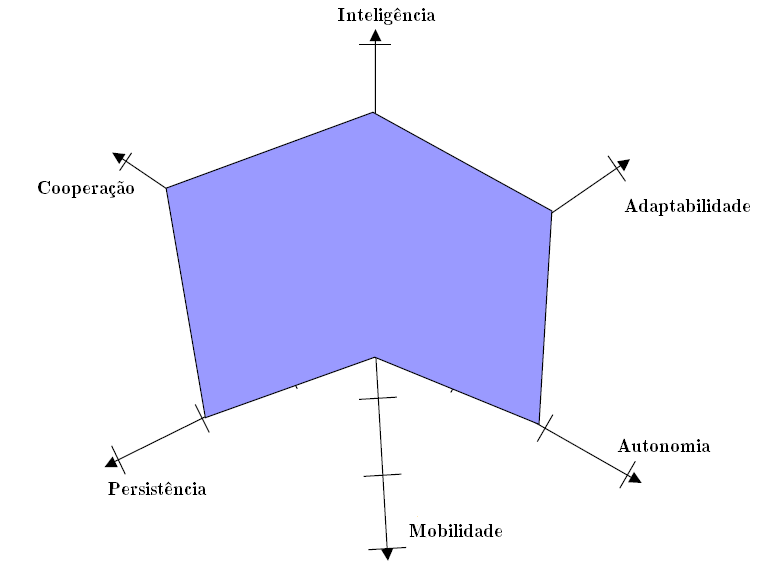
\includegraphics[scale=0.7]{figuras/hexagono_agente}
    \centering
    \caption{Dimensões do agente. Fonte: \cite{griss2001software}. Traduzido.}
    \label{fig:hexagono}
\end{figure}

\section{Sistemas Multiagentes}

Sistemas multiagentes se enquadram no cenário onde coexistem dois ou mais agentes. Seus objetivos individuais  correspondem a subpartes de que do objetivo geral do sistema \cite{mcarthur2007multi}.

Torna-se necessário para um agente representar e raciocinar sobre os outros agentes no ambiente \cite[pág. 887]{van2008handbook}. 


\section{Padrão}

\section{Arquitetura de Sistemas Multiagentes}



